\documentclass[a4paper]{article}
\usepackage[left=2cm,right=2cm,top=2cm,bottom=2cm]{geometry}
\usepackage[utf8]{inputenc}
\usepackage{indentfirst}
\usepackage{graphicx}
\usepackage{hyperref}
\usepackage{caption}
\usepackage{subcaption}
\usepackage{multirow}
\renewcommand{\thesection}{\Roman{section}}

\hypersetup{colorlinks=true, urlcolor=blue ,citecolor=blue}


\title{ \huge{\textbf{CRC - 1st Project Report}} \\
        \Large{Studying the Marvel Universe Network}}

\author{
  Afonso Ribeiro, 86752\\ Andreia Pereira, 89414\\ Pedro Nunes, 89525
}

\date{October 2020}

\begin{document}
\maketitle

\begin{abstract}
This is a project in the context of our Network Science course. We studied the Marvel Universe collaboration network, where two characters are linked if they appear in at least one common Marvel comic book. The goal of this project is to study the properties of this network and, possibly, infer some interesting conclusions about it.
\end{abstract}

\section{Introduction}\label{intro}

Collaboration networks are found everywhere in our lives. In these networks, the nodes represent people and, if two nodes are connected, it means that there is some sort of collaboration between them. Friendships in social networks, scientific collaborations in papers, or even co-appearances in Hollywood movies are examples of very palpable collaboration networks. While our network does not represent real people, it portraits social interactions between characters in books, that, as we found out, somewhat resembles real friendship networks.

Our Marvel Universe network is based on a data set assembled by \cite{cond-mat} . The original data set links Marvel characters to the books in which they appear. We then processed this data set to better suit our purposes. In our network, each node node represents a Marvel character and two nodes are linked if they appear in at least one common comic book.

We developed our project using the NetworkX framework for Python. The network is parsed and translated to a NetworkX Graph structure, which then we use to evaluate the network. While we used some built-in functions for NetworkX to more efficiently calculate some network parameters, we chose to develop some basic code to analyse and visualize it.

\section{Results}\label{res}
Our Marvel network has 6486 nodes and 168267 edges. The network is composed of one large connected component containing 6449 nodes, and the remaining 37 nodes are isolated. In the Marvel Universe, this means that there are 37 characters that never appear with any other character in a comic book. 
In the following table we present some of the metrics calculated for the network.

\subsection{Metrics}
\begin{center}
\begin{tabular}{ r | c }
 Average Degree & 51.89 \\[5pt]
 Average Clustering Coefficient & 0.77\\[5pt]
 Size of the Largest Connected Component (LCC) & 6449 \\[5pt]
 Average Path Length of the LCC & 2.63 \\[5pt]
 Diameter of the LCC & 5 \\[5pt]
 
\end{tabular}
\end{center}
%Avg. Degree, avg. path length, avg. clustering coefficient, diameter, Pk, centrality, largest component, largest hub (c/ imagem)
\subsection{Distances}
The Average Degree of the Marvel network is 51.89, meaning that, on average, a Marvel character co-appears in comic books with almost 52 different characters. 
To evaluate how far each character is from each other, we only considered the largest connected component. This is a fair approximation since it contains to 99.4\% of the nodes. We find that, on average, each character is 2.63 leaps away to every other character - this is given by the Average Path Length. The small world phenomenon implies that the distance between two randomly chosen nodes in a network is short \cite{Network Science}. By this definition, we can argue that the Marvel Network is a small world. We also find that the maximum distance between two characters is only 5 edges. 

\subsection{Power Law}
The Marvel network is far from being a random network. Its degree distribution much more closely resembles a Power Law. We developed various functions that analyse the degree distribution and allow us to better visualize it. We used the Scipy library to fit our distribution to a Power Law curve. Here we present our attempt in doing so.


\begin{figure}[h!]
\centering
\begin{subfigure}{.5\textwidth}
  \centering
  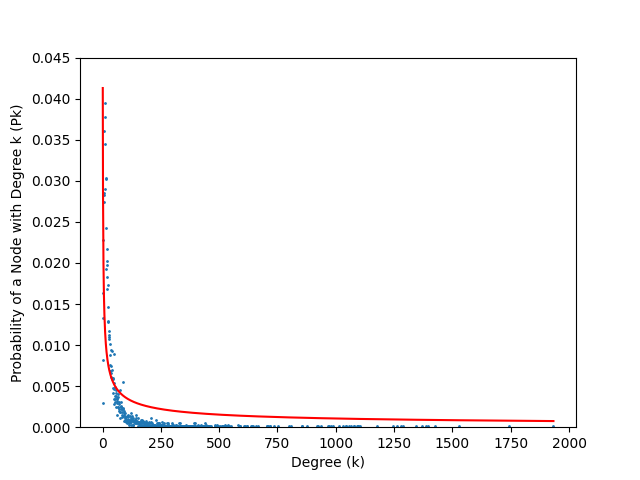
\includegraphics[width=0.9\linewidth]{pl_linear_non_adjusted}
  \caption{Degree Distribution on a Linear Scale.}
  \label{fig:pl_linear_non_adjusted}
\end{subfigure}%
\begin{subfigure}[h!]{.5\textwidth}
  \centering
  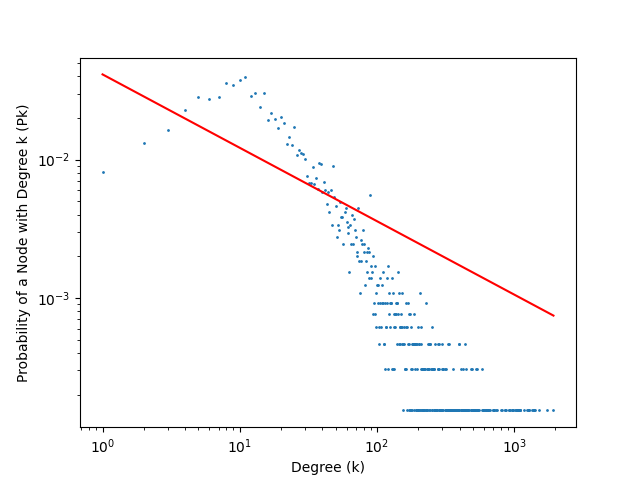
\includegraphics[width=0.9\linewidth]{pl_log_non_adjusted}
  \caption{Degree Distribution on a Logarithmic Scale.}
  \label{fig:pl_log_non_adjusted}
\end{subfigure}
\caption{Power Law fitted to all degree values .\\ $Pk =0.0413*k^{-0.530}$ }
\label{fig:pl_non_adjusted}
\end{figure}

\begin{figure}[h!]
\centering
\begin{subfigure}[h!]{.5\textwidth}
  \centering
  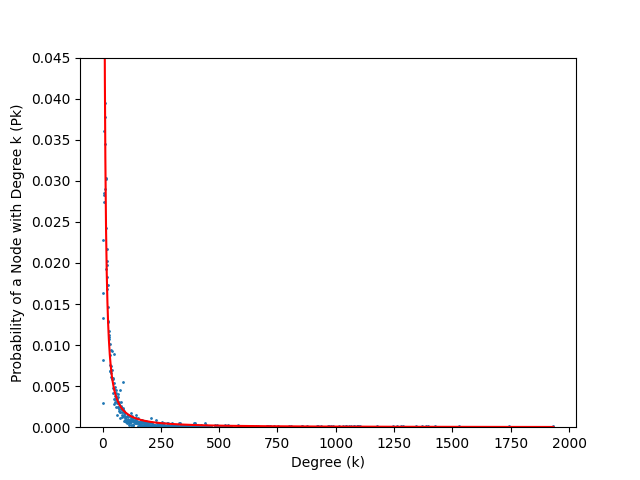
\includegraphics[width=0.9\linewidth]{pl_linear_adjusted}
  \caption{Degree Distribution on a Linear Scale.}
  \label{fig:pl_linear_adjusted}
\end{subfigure}%
\begin{subfigure}{.5\textwidth}
  \centering
  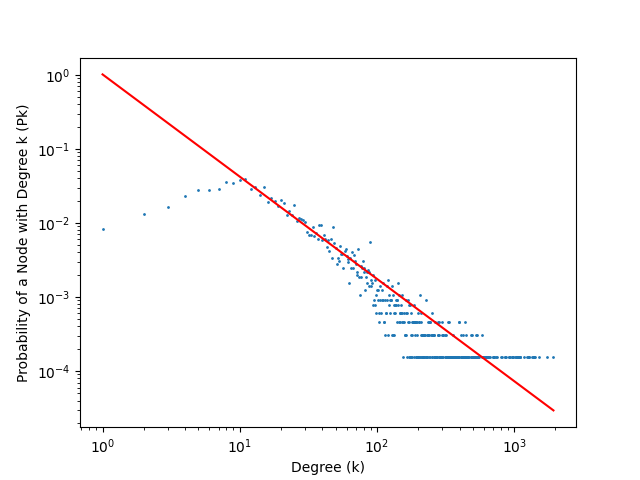
\includegraphics[width=0.9\linewidth]{pl_log_adjusted}
  \caption{Degree Distribution on a Logarithmic Scale.}
  \label{fig:pl_log_adjusted}
\end{subfigure}
\caption{Power Law fitted to degree values $>$ 9.\\  $Pk =1.014*k^{-1.381}$}
\label{fig:pl_adjusted}
\end{figure}

We found out that a Power Law does not describe our network for the first values of degrees (i.e. for k between 0 and 9). Our explanation for this phenomenon is that in a comic book series there aren't that many characters that don't interact with lots of other characters. In a perfect Power Law distribution, the majority of nodes would have very few links, so a node with degree 0 or 1 would be the most common. However, in a book universe, it is natural not to find this property, as the characters tend to collaborate with each other (it is very rare to find a book that only has one or two characters). 
Due to this, we ignored the first 10 degree values to fit the Power Law curve. This adjustment is shown in figure~\ref{fig:pl_adjusted}, where it is visible that it is a much better adjusted to our distribution.

Analysing this adjusted Power Law function, we notice that  $\lambda = 1.381 < 2$. This means that our network falls under the Anomalous Regime \cite{Network Science}. One conclusion might be that this Marvel network can't grow much bigger, as when $N \rightarrow +\infty$, $<k>$ diverges. However, in a small network like ours, a $\lambda < 2$ might mean that the average properties of the network are much more heavily determined by the nodes with the largest degrees\cite{cond-mat}. 


\subsection{Centrality and Hubs}
We opted to analyse the centrality of the Marvel network's nodes as if we were dealing with a real-life social network. In the topic of social networks, we chose three relevant centrality measures, namely the Degree Centrality (DC), the Closeness Centrality (CC), and the Betweenness Centrality(BC) \cite{cent_meas}. Here we present the top-3 characters with the biggest values of each centrality measure.

\bigskip

\begin{center}
\setlength{\tabcolsep}{10pt} % Default value: 6pt
\renewcommand{\arraystretch}{1.2} % Default value: 1
\begin{tabular}{ |c|c|c| } 
\hline
{Centrality Measures(CM)}
& Character Names & CM Values\\
\hline
\multirow{3}{*}{Degree Centrality (DC)}
& SPIDER-MAN/PETER PARKER & 0.298 \\
& CAPTAIN AMERICA & 0.268 \\
& IRON MAN/TONY STARK & 0.236\\

\hline
\multirow{3}{*}{Closeness Centrality (CC)}
& SPIDER-MAN/PETER PARKER & 0.583 \\
& CAPTAIN AMERICA & 0.572 \\
& IRON MAN/TONY STARK & 0.560\\
\hline
\multirow{3}{*}{Betweenness Centrality (BC)}
& SPIDER-MAN/PETER PARKER & 0.073 \\
& CAPTAIN AMERICA & 0.057 \\
& HAVOK/ALEX SUMMERS & 0.043\\

\hline
\end{tabular}
\end{center}


\bigskip

With DC, the number of a network member’s direct contacts is a useful indicator of centrality. We assume that this measure is a generic measure of popularity. The conclusion that Spider-Man, Captain America and Iron Man have the highest DC does not come as a shock, as they are intuitively the most popular super-heroes. 

The CC can be used to find what characters are able to disseminate information on the network more effectively. These are the nodes that have a short distance to other nodes, requiring few intermediaries to contact other nodes. This further confirms our most popular super-heroes are Spider-Man, Captain America and Iron Man.

At last, BC indicates what nodes are important to establish the flow of the network, serving as bridges between hubs. This might be the most relevant measure in our case, as it highlights the Marvel characters that link multiple story lines. We found out that while Iron Man is more popular than Havok, the lather is more crucial to connecting the network. It makes sense that none of the super-heroes has a high BC value. Our network is saturated, meaning that there are no clusters or very separated hubs. It can be treated as a large hub in which some super-heroes have a high influence.

\section{Discussion}\label{disc}
Our main goal was to compare the Marvel network to real-life collaboration networks. The Marvel network is a artificial network that was built by book writers with no particular goals of truthfully representing a human collaboration network. However, we have found that the Marvel network has common properties of real collaboration networks. Its degree distribution shows a clear power-law tail with cutoff. Additionally, the short distance between characters is a powerful property to take into consideration, as it confirms the small world phenomenon. A measure that contradicts this comparison is the clustering coefficient of the network, that is much smaller than in real-life social networks\cite{cond-mat}.

Real collaboration networks have common properties, namely being ruled by a power law distribution and being small worlds. Through this lens, we can safely conclude that the Marvel network resembles a real collaboration network in spite of its artificial nature.



\begin{thebibliography}{10}
\bibitem{cond-mat}R. Alberich, J. Miro-Julia, F. Rossello, Marvel Universe looks almost like a real social network, Cornell University \url{https://arxiv.org/abs/cond-mat/0202174}

\bibitem{Network Science}Barabási, A.-L., Network Science, 2016, Cambridge University Press \url{http://networksciencebook.com}

\bibitem{cent_meas}A Critical Review of Centrality Measures in Social Networks \url{https://link.springer.com/article/10.1007/s12599-010-0127-3}

\end{thebibliography}

\end{document}
